\chapter{Computational approach}
\label{ch:computational-approach}

In order to find a counter-example to the Krenn's conjecture in the best case scenario, or just to find interesting new properties in perfectly monochromatic graphs, having a more experimental approach has many interests.
In this section, I am introducing a new tool I developed, called EGPI, that computes the weighted matching index of experiment graphs.
Then, some of its potential uses are presented.

\section{Motivation}
\label{sec:computational-motivations}

Finding interesting examples of experimental graphs to study can be challenging due to the high degree of freedom experiment graphs can have, by definition~\ref{def:experiment_graph}.
Also, the weighted matching index of experiment graphs as defined in definition~\ref{def:weighted_matching_index} is hard to find by hand since it requires finding all perfect matchings of a graph.
In my knowledge, no public access tool exists at the time of writing to easily encode experimental graphs and compute their weighted matching index.
My hope is that such a tool could help me and other researchers to quickly verify some properties on instances of graphs they want to test, without losing more time on it.
For this reason, I developed a new program that does exactly that.
The program is called \textbf{EGPI}, which stands for \textbf{Experiment Graphs Properties Identifier}.
I believe this name resumes the whole meaning of its utilization.
The program is available on my Github repository~\cite{githubEGPI}.


\section{Limitations of the experimental approach}
\label{sec:egpi-limitations}

Assuming that we successfully find a way to compute in a quick time the weighted matching index of an experiment graph, we still have to face some limitations.
It may be tempting to use such a tool to prove the conjecture in some very restrained cases by generating and testing every possible experiment graph that respects some properties.
While this idea is theoretically possible, the user must be aware that he is extremely limited by the computational time of such an algorithm.
Indeed, the number of possible graphs grows exponentially with their degrees of freedom.\\

Let's consider a quick and simple example by trying to prove experimentally the following conjecture.

\begin{conjecture}
    \label{con:krenn_6}
    Let $G_k^w$ be a non-redundant experiment graph of size $n = 6$ vertices, and let say that, for all edge $e \in E(G)$,
    \begin{center}
        $\left\{\begin{array}{l l}
            Re(w(e)) & \in \{-1, 0, 1\} \\
            Im(w(e)) & \in \{-1, 0, 1\} \\
            w(e)     & \neq 0          \\
        \end{array}\right.$
    \end{center}
    Then, the weighted matching index $\Tilde{c}(G, k, w) \leq 2$.
\end{conjecture}

One way to prove the conjecture~\ref{con:krenn_6} is to use a brute force algorithm that generates every possible graph respecting the pre-conditions of the conjecture~\ref{con:krenn_6} with bicoloured edges that can take their colours in $3$ defined colours $(r, g, b)$, and check their weighted matching index.
If none of their weighted matching index is $3$, then the conjecture is true.
Unfortunately, this is not possible because of the following observation.\\

\begin{observation}
    Let $G_k^w$ be an experiment graph that has $n$ vertices, and let say that, for all edge $e = (u, v) \in E(G)$, the edge can have a value different from $0$ chosen among $W$ different values.
    Furthermore, $k(e, u)$ and $k(e, v)$ are chosen among $K$ different colours.
    At last, $\forall e' = (u, v), k(e') \neq k(e)$.
    Then, the number of different possible graphs that $G_k^w$ can be, denoted $N_{graphs}$, is

    \begin{center}
        $N_{graphs} = (1 + W)^{\left(\frac{K^2 \cdot n \cdot (n-1)}{2}\right)}$
    \end{center}
\end{observation}


\begin{proof}
    Indeed, each edge $e$ is characterized by the following properties.
    \begin{itemize}
        \item It has a position $\{u, v\}$, that can take $\frac{n \cdot (n -1)}{2}$ different values.
        \item It has $2$ colours, one at each of its endpoint, that can take $K$ different values.
            Then, in total, there are $K^2$ different ways to bicolour it.
        \item It has a complex weight that can have $W$ different value.
    \end{itemize}

    A first observation is that the maximum number of edges between $2$ different nodes of $V(G)$ is $K^2$.
    Indeed, more edges would imply that $2$ edges at least would have the same positions and colours, which is forbidden.\\

    Then, we observe that there are $W^x$ possibilities to assign weights to an edge set of size $x$.
    Using these $2$ last observations, it is possible to compute the number of different weighted bicoloured edges sets between $2$ defined nodes $u$ and $v$.
    Let's denote this number $N_{edges}$.

    \begin{center}
        $\begin{array}{r c l}
             N_{edges} & = & {K^2 \choose 0} W^0 + {K^2 \choose 1} W^1 + {K^2 \choose 2} W^2 + \cdots + {K^2 \choose K^2} W^{K^2} \\
                       & = & \sum\limits_{x=0}^{K^2} {K^2 \choose x} W^x
        \end{array}$
    \end{center}

    It is possible to simplify this expression by using the binomial theorem~\cite{wikipediaBinomialTheorem}.

    \begin{center}
        $\begin{array}{r c l}
             N_{edges} & = & \sum\limits_{x=0}^{K^2} {K^2 \choose x} W^x               \\
                       & = & \sum\limits_{x=0}^{K^2} {K^2 \choose x} 1^{(K^2 - x)} W^x \\
                       & = & (1 + W)^{K^2}
        \end{array}$
    \end{center}

    Having this number, it is easy to find the number $N_{graphs}$ of possible experiment graphs.
    Indeed, we just have to choose one of the possible combinations of weighted bicoloured edges between $2$ defined nodes for each possible pair of nodes.
    The number of possible pairs of nodes is $\frac{n \cdot (n-1)}{2}$.
    Therefore:

    \begin{center}
        $\begin{array}{r c l}
             N_{graphs} & = & N_{edges} ^ {\frac{n \cdot (n-1)}{2}}                  \\
                        & = & \left((1 + W)^{K^2}\right)^{\frac{n \cdot (n-1)}{2}}   \\
                        & = & (1 + W)^{\left({K^2} \cdot \frac{n \cdot (n-1)}{2}\right)} \\
        \end{array}$
    \end{center}
\end{proof}

Returning to conjecture~\ref{con:krenn_6}, let's compute as an example the number of graphs needed to verify to prove it by a brute force algorithm.
The graphs described in conjecture~\ref{con:krenn_6} have $n = 6$ vertices, $K = 3$ different possible colours per edge's endpoint, and $W = 8$ possible weights different from $0$.
Therefore, in this case,

\begin{center}
    $\begin{array}{r c l}
         N_{graphs} & = & (1 + W)^{\left(\frac{K^2 \cdot n \cdot (n-1)}{2}\right)} \\
                    & = & (1 + 8)^{\left(\frac{3^2 \cdot 6 \cdot (6-1)}{2}\right)} \\
                    & = & 9^{270}
    \end{array}$
\end{center}

This number is absurdly big, and it is totally impossible to imagine being able to generate all of those graphs on a classical computer and compute their matching index, no matter of how efficient this operation is.
Therefore, conjecture~\ref{con:krenn_6} cannot be solved by using a brute force algorithm, even if the graphs it is about are tiny and restricted compared to the space of all experiment graphs possible.\\

This observation leads us to consider that EGPI, in its implementation, should not try to generate all possible graphs.
Instead, it should focus on generating as wisely as possible random graphs that have a high probability to have a big weighted matching index.
This is the approach I took in the development of EGPI, and it is detailed in the next subsections.


\section{Functionalities of EGPI}
\label{sec:functionalities-of-egpi}

At the current state of its development, EGPI implements functions that allow the user to do the following:

\begin{enumerate}
    \item \textbf{Discover all the perfect matchings of an encoded experiment graph}.
        The perfect matchings are encoded as edge sets.
        Their encoding includes access to their weights and to the feasible vertex colouring they induce.
    \item \textbf{Discover all the feasible vertex colourings of an encoded experiment graph}.
        The set of all feasible vertex colourings of a graph is encoded as a Python dictionary, where the vertex colourings (Python tuples) are the keys and their weights (complex numbers) are the values.
    \item \textbf{Find out if an encoded experiment graph is perfectly monochromatic or not.}
    \item \textbf{Compute the weighted matching index of an encoded experiment graph.}
    \item \textbf{Find out if an encoded experiment graph is bipartite.}
    \item \textbf{Save an encoded experiment graph and its properties in a JSON file.}
        The JSON file contains all the properties of the graph, including its perfect matchings, its feasible vertex colourings, its weighted matching index, and the fact it is bipartite or not.
    \item \textbf{Draw an encoded experiment graph in a pdf file.}
        This is done through the creation of a tex file containing the LaTeX representation of the graph.
        This LaTeX file is still available after the program ends, so that its code can be re-used if wanted so.
    \item \textbf{Randomly create candidate experiment graph}, a process that can be defined as follows.
        \begin{definition}[Random creation of a candidate experiment graph]
            \label{def:random-creation-candidate-experiment-graph}
            Given an even number of nodes $n \in \mathbb{N}$, a list of colours $L_{colours}$, a list of complex numbers $L_{weights}$, and a complexity bound $b \in \mathbb{N}$, the \textit{random creation of a candidate experiment graph} respecting $n$, $L_{colours}$, $L_{weights}$ and $b$ is the process described in algorithm~\ref{alg:random_creation_candidate_experiment_graph}.

            \begin{algorithm}
                \caption{Random creation of a candidate experiment graph}
                \label{alg:random_creation_candidate_experiment_graph}
                \begin{algorithmic}
                    \Require $n$ is a positive even integer
                    \Require $L_{colours}$ is a list of colours
                    \Require $L_{weights}$ is a list of complex numbers different from 0
                    \Require $b \in \mathbb{N}$
                    \State $G_k^w \gets$ an empty graph with $n$ vertices and no edge
                    \For {$k \in L_{colours}$}
                        \State $S \gets \frac{n}{2}$ non-touching edges at random positions of $G_k^w$
                        \State Colour each edge $\in S$ with colour $k$
                        \State Assign random weights $\in L_{weights}$ to each edge $\in S$
                        \State Add $S$ to $E(G_k^w)$
                        \Comment{These edges form a monochromatic perfect matching}
                    \EndFor

                    \For {$i \in \{1, 2, \dots, b\}$}
                        \State $S \gets \frac{n}{2}$ non-touching edges at random positions of $G_k^w$
                        \For {each pair of vertices $(u, v) \in S$}
                            \If {there is no edge between $u$ and $v$ in $G_k^w$}
                                \State Add an edge $e$ between $u$ and $v$
                                \State Colour $e$ with a bicolour $\in L_{colours}^2$
                                \State Assign a weight $\in L_{weights}$ to $e$
                            \Else
                                \State $add\_edge \gets True$ with probability $\frac{1}{(\mbox{\#edges between u and v}) + 1}$
                                \If {$add\_edge$}
                                    \State Add an edge $e$ between $u$ and $v$
                                    \State Colour $e$ with a bicolour $\in L_{colours}^2$ different from the bicolour of the other edges between $u$ and $v$
                                    \State Assign a weight $\in L_{weights}$ to $e$
                                \EndIf
                            \EndIf
                        \EndFor
                    \EndFor
                \end{algorithmic}
            \end{algorithm}
        \end{definition}

    The denomination \textit{candidate} experiment graph comes from the fact that graphs built that way have higher chances to have big weighted matching index than completely random graphs.
    Also, this construction ensures that each of the edges included in a candidate graph is part of a perfect matching.
    Furthermore, they do not have multiple edges of the same bicolour between $2$ vertices.
    Assuming $0 \in L_{weights}$, this makes them non-redundant, according to the definition~\ref{def:non_redundant_induced_subgraph}.
    All of these observations make them indeed good \textit{candidates} to study.

    \item \textbf{Perform a random experiment graphs research process}, defined as follows.
        \begin{definition}[Random Experiment Graphs Research Process]
            \label{def:random_experiment_graphs_research_process}
            Given a number of nodes $n \in \mathbb{N}$, a list of colours $L_{colours}$, a complexity bound $b \in \mathbb{N}$, a list of complex numbers $L_{weights}$, and a number of trials $m \in \mathbb{N}$, a \textit{Random Experiment Graphs Research Process} is the process of randomly creating $m$ candidate experiment graphs respecting $n$, $L_{colours}$, $L_{weights}$ and $b$, and analyse them.
            More specifically, each of these graphs $G_k^w$ gets verified to check if it is perfectly monochromatic and if it has at least one non-monochromatic feasible vertex colouring.
            If it is, $G_k^w$ is saved as a JSON file containing all its properties (including its perfect matchings, its feasible vertex colourings, its weighted matching index, and the fact it is bipartite or not).
            Then, $G_k^w$ is drawn in another pdf file.
        \end{definition}

        In short, this experiment allows the user to generate a big number of experiment graphs and analyse properties on them.
        The condition that the graphs must have at least one non-monochromatic feasible vertex colouring allows the user to focus on non-trivial graphs.
        Indeed, if it is not satisfied, then the graph is monochromatic, according to definition~\ref{def:monochromatic_graph}, and this case of the Krenn's conjecture is already proven thanks to Bogdanov~\cite{bogdanov}.

\end{enumerate}


\section{Details of implementation}
\label{sec:details-of-implementation}

This section explains all the technical aspects of the implementation of EGPI\@.
Readers only interested in its use can pass this section if they want to.\\

EGPI was implemented in Python, this choice was motivated by two reasons.
Firstly, Python is a high-level programming language that offers many functionalities and data types by default~\cite{python}.
This made the implementation a lot easier and compacter than if it had to be done in other programming languages.
Secondly, Python is easy to read and to learn for people who are not familiar with programming.
This may allow future researchers interested in re-using EGPI to perform modifications to it without too many difficulties if they want to.\\

The main purpose of EGPI is to encode and apply operations on experiment graphs, rigorously defined in definition~\ref{def:experiment_graph}.
It is therefore important to build a good data structure of experiment graphs.
The architecture of the program to do so is detailed in a state diagram available in figure~\ref{fig:structure_diagram}.

\begin{figure}[H]
    \centering
    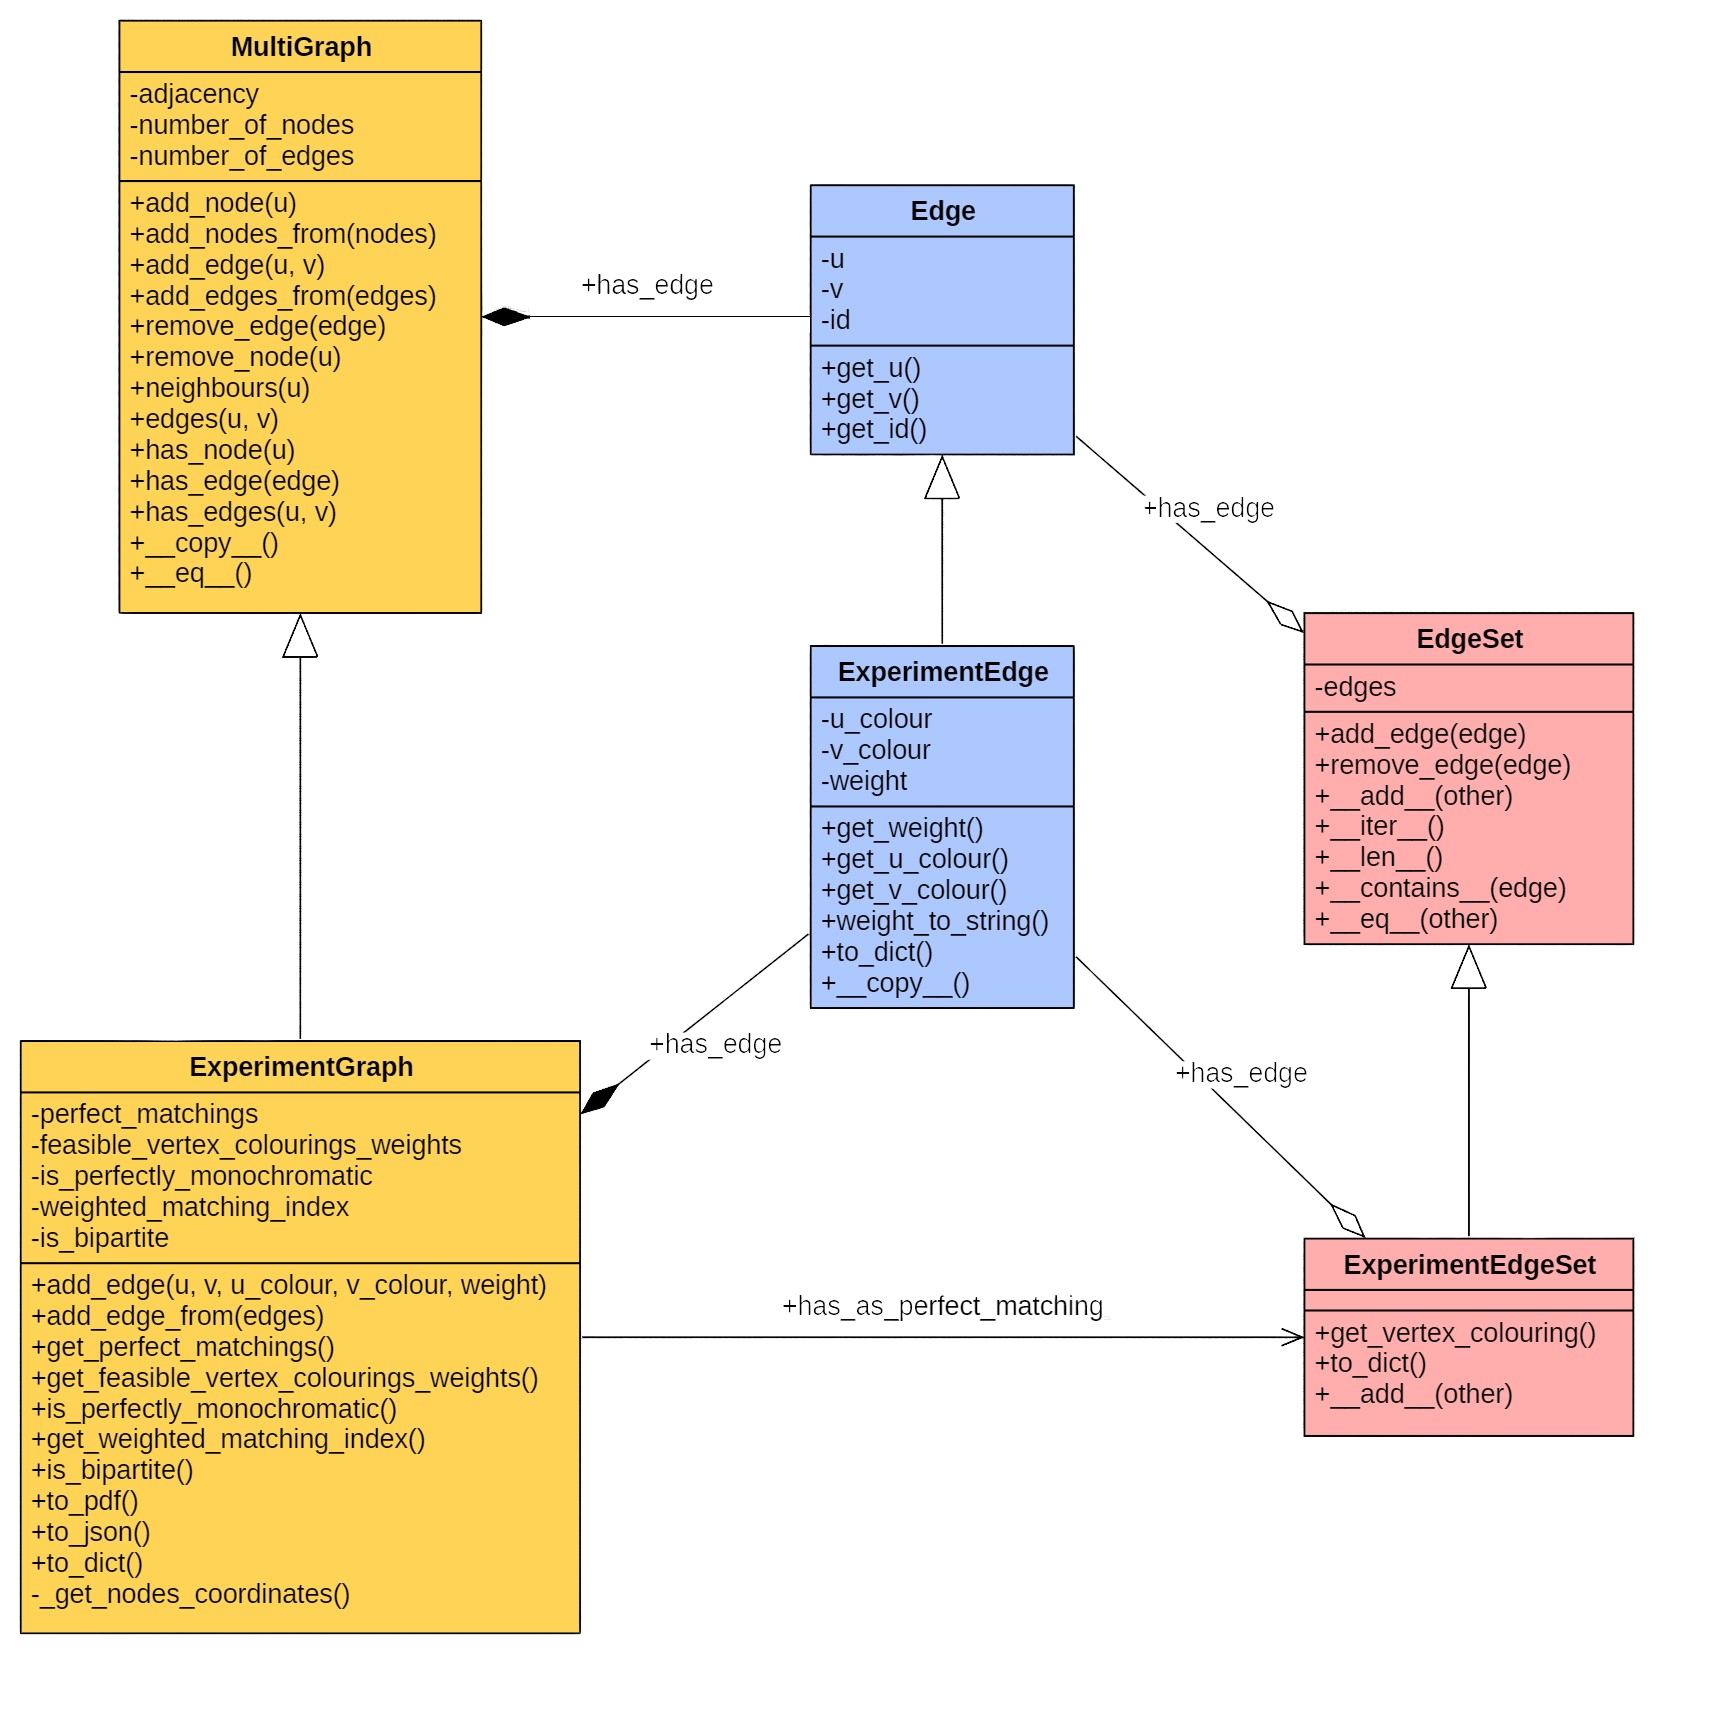
\includegraphics[scale=0.25]{figures/new_results/egpi/structure_diagram}
    \caption{Structure diagram of EGPI showing the important relations between the different implemented data structures. Most of the implemented methods of the program are shown in the diagram.}
    \label{fig:structure_diagram}
\end{figure}

Here is an exhaustive list of all non-trivial experiment graphs' properties we are interested to compute, and the algorithms we use in EGPI to do so.

\begin{enumerate}
    \item \textbf{Their perfect matchings:} to find all the perfect matchings of a graph, EGPI uses an algorithm written in pseudocode in algorithm~\ref{alg:perfect_matchings}.

        \begin{algorithm}
            \caption{Find all perfect matchings of an experiment graph $G$}
            \label{alg:perfect_matchings}
            \begin{algorithmic}
                \Require $G$ is an experiment graph
                \If{$G$ has no node}
                    \State The only perfect matching is $\varnothing$
                \ElsIf{$G$ has nodes}
                    \State $PMs$ $\gets$ empty list
                    \State choose a random node $u \in V(G)$
                    \ForAll{$v \in$ neighbours of $u$}
                        \State $subPMs \gets$ all perfect matchings of $G$ without $u$ and $v$
                        \ForAll{$subPM \in subPMs$}
                            \ForAll{$e \in$ edges between $u$ and $v$}
                                \State add $subPM \cup e$ to $PMs$
                            \EndFor
                        \EndFor
                    \EndFor
                \EndIf
                \State \Return PMs
            \end{algorithmic}
        \end{algorithm}

        \paragraph{Complexity of algorithm \ref {alg:perfect_matchings}:}
        The algorithm is a depth first search (DFS) algorithm.
        In the worst case scenario, $G_k^w$ is a complete graph with $n$ vertices.
        In other words, each node has $n-1$ neighbours in $G_k^w$.
        Also, at each recursive step of the algorithm, we remove $2$ nodes from the graph.
        This means that the depth of the search tree is $\frac{n}{2}$.
        The running time of this search algorithm is then $O\left(n^\frac{n}{2}\right)$. \\

    \item \textbf{The weights of their feasible vertex colourings:} according to their definition~\ref{def:feasible_vertex_colouring}, finding the feasible vertex colourings of an experiment graph requires to find their perfect matchings.
        The next steps to find them and their weights are simpler and are described in algorithm~\ref{alg:feasible_vertex_colourings}.

        \begin{algorithm}
            \caption{Find all feasible vertex colourings of an experiment graph $G_k^w$}
            \label{alg:feasible_vertex_colourings}
            \begin{algorithmic}
                \Require $G_k^w$ is an experiment graph
                \State $PMs \gets$ all perfect matchings of $G_k^w$
                \State $FVCs \gets$ empty Python dictionary
                \ForAll{$PM \in PMs$}
                    \State $FVC \gets$ feasible vertex colouring induced by $PM$
                    \State $w \gets$ weight of $PM$
                    \State $FVCs[FVC] \gets w$
                \EndFor
                \State \Return $FVCs$
            \end{algorithmic}
        \end{algorithm}

        The hardest step of this algorithm is to find all the perfect matchings of $G_k^w$.
        Therefore, the complexity of this algorithm is the same as the one of algorithm~\ref{alg:perfect_matchings}, which is $O\left(n^\frac{n}{2}\right)$ in the worst case.

    \item \textbf{If the graph is perfectly monochromatic:} by definition~\ref{def:perfectly_monochromatic_graph}, finding if an experiment graph is perfectly monochromatic or not just requires looking at all its feasible vertex colourings.
        This is done in algorithm~\ref{alg:perfectly_monochromatic}.

        \begin{algorithm}
            \caption{Check if an experiment graph $G_k^w$ is perfectly monochromatic}
            \label{alg:perfectly_monochromatic}
            \begin{algorithmic}
                \Require $G_k^w$ is an experiment graph
                \State $FVCs \gets$ all feasible vertex colourings of $G$
                \State $isPM \gets$ True
                \ForAll{$FVC \in FVCs$}
                    \If{FVC is monochromatic and $w(FVC) \neq 1$}
                        \State $isPM \gets$ False
                    \ElsIf{FVC is not monochromatic and $w(FVC) \neq 0$}
                        \State $isPM \gets$ False
                    \EndIf
                \EndFor
                \State \Return $isPM$
            \end{algorithmic}
        \end{algorithm}

        The only hard step of this algorithm is to find all the feasible vertex colourings of $G_k^w$.
        Therefore, the complexity of this algorithm is the same as the one of algorithm~\ref{alg:feasible_vertex_colourings}, which is $O\left(n^\frac{n}{2}\right)$ in the worst case.

    \item \textbf{The weighted matching index of the graph:} defined in definition~\ref{def:weighted_matching_index}, the weighted matching index of a perfectly monochromatic experiment graph is the number of monochromatic feasible vertex colourings in this graph.
        If the graph is not perfectly monochromatic, the weighted matching index is $0$ by definition.
        EGPI uses the algorithm~\ref{alg:weighted_matching_index} to compute the weighted matching index of a graph.
        \begin{algorithm}
            \caption{Compute the weighted matching index of an experiment graph $G_k^w$}
            \label{alg:weighted_matching_index}
            \begin{algorithmic}
                \Require $G_k^w$ is an experiment graph
                \State $FVCs \gets$ all feasible vertex colourings of $G_k^w$
                \State $isPM \gets$ is $G_k^w$ perfectly monochromatic ?
                \If{$isPM$}
                    \State $c \gets 0$
                    \ForAll{$FVC \in FVCs$}
                        \If{$w(FVC) = 1$}
                            \State $c \gets c + 1$
                        \EndIf
                    \EndFor
                    \State \Return $c$
                \Else
                    \State \Return $0$
                \EndIf
            \end{algorithmic}
        \end{algorithm}

        Again, the complexity of this algorithm is determined by the one of algorithm~\ref{alg:feasible_vertex_colourings}, which is $O\left(n^\frac{n}{2}\right)$ in the worst case.

    \item \textbf{If the graph is bipartite:} finding if a graph is bipartite or not is a well-known problem in graph theory.
        EGPI uses the following greedy algorithm to find if a graph is bipartite or not.
        The algorithm is written in algorithm~\ref{alg:bipartite}.
        \begin{algorithm}
            \caption{Check if an experiment graph $G_k^w$ is bipartite}
            \label{alg:bipartite}
            \begin{algorithmic}
                \Require $G_k^w$ is an experiment graph
                \State $Q \gets$ empty queue
                \State add $v_0 \in V(G_k^w)$ to $Q$
                \State colour of $v_0 \gets$ red
                \State $isBipartite \gets$ True
                \While{$Q$ is not empty}
                    \State $u \gets$ pop $Q$
                    \ForAll{$v \in$ neighbours of $u$}
                        \If{colour of $v$ is not defined}
                            \State colour of $v \gets$ opposite colour of $u$
                            \State add $v$ to $Q$
                        \ElsIf{colour of $v$ is the same as colour of $u$}
                            \State $isBipartite \gets$ False
                        \EndIf
                    \EndFor
                \EndWhile
                \State \Return $isBipartite$
            \end{algorithmic}
        \end{algorithm}

        This algorithm visits all the nodes of $G_k^w$ only once.
        Therefore, its complexity is $\mathcal{O}(n)$, where $n$ is the number of vertices of $G_k^w$.

\end{enumerate}


\section{Realized experiments with EGPI}
\label{sec:realized_experiments}

In this section, I present some of the experiments I realized with EGPI. The goal of these experiments was to find interesting properties of experiment graphs, and to try to find a counter-example to the Krenn's conjecture.\\

\subsection{Research for counter-examples}
\label{subsec:research-for-counter-examples}

The first experiment I realized with EGPI was to try to find a counter-example to the Krenn's conjecture.
To do so, I performed different random experiment graphs research processes, defined in definition~\ref{def:random_experiment_graphs_research_process}.
Each of these processes used the following parameters.

\begin{itemize}
    \item The number of trials was $m = 10^6$.
    \item The possible colours of the edges were $L_{colours} = \{red, green\}$.
    \item The possible complex weights of the edges were $L_{weights} = \{-1, 1, -i, i\}$.
\end{itemize}

I performed $21$ different random experiment graphs research processes, with $n \in {6, 8, 10}$ and $b \in \{1, 2, 3, 4, 5, 6\}$.

On all the $21$ millions generated candidate graphs, none of them was perfectly monochromatic.
This result is a new argument in favour of the Krenn's conjecture, at least for graphs that have less than $10$ vertices.
Nevertheless, it does not constitute a proof of it in any case, and I encourage future researchers to continue looking for counterexamples to it alongside their researches (by using EGPI or any other tool). \\


\subsection{Research for perfectly monochromatic graphs with a weighted matching index of $2$}
\label{subsec:research-for-graphs-with-c-of-2}

The second experiment I realized with EGPI was to try to find perfectly monochromatic graphs that have a weighted matching index of $2$.
These graphs are authorized by the Krenn's conjecture, and their properties are interesting to study.
Indeed, understanding better the structure of these graphs might help researchers to find new ideas in their seek for a proof to the conjecture.\\

But this is not the main and only interest of the experiment.
Exploring this class of experiment graphs is a great way to test the different functionalities of EGPI, and to experimentally check the impact of the different parameters of the program.
Using the following parameters,

\begin{itemize}
    \item The number of trials was $m = 10^6$.
    \item The possible colours of the edges were $L_{colours} = \{red, green\}$.
    \item The possible complex weights of the edges were $L_{weights} = \{-1, 1, -i, i\}$.
\end{itemize}

I performed $15$ different random experiment graphs research processes, with $n \in {6, 8, 10}$ and $b \in \{1, 2, 3, 4, 5\}$.
I got results summarized in figure~\ref{fig:results-experiment}.

\begin{figure}[H]
    \centering
    \begin{tabular}{ |p{1cm}||p{1.5cm}|p{1.5cm}|p{1.5cm}|p{1.5cm}|p{1.5cm}|p{1.5cm}|  }
        \hline
        \multicolumn{7}{|c|}{Results of the experiment} \\
        \hline
        $n$ & $b = 1$ & $b = 2$ & $b = 3$ & $b = 4$ & $b = 5$ & total \\
        \hline
        $6 $ & $103$ & $18$ & $4$ & $0$ & $0$ & $125$ \\
        $8 $ & $39$  & $1$  & $0$ & $0$ & $0$ & $40$  \\
        $10$ & $3$   & $0$  & $0$ & $0$ & $0$ & $3$   \\
        \hline
    \end{tabular}
    \caption{Results of $3$ different random experiment graphs research process with $n=6$, $n=8$ and $n=10$ respectively.}
    \label{fig:results-experiment}
\end{figure}

Here is an example of discovered perfectly monochromatic graph by the program.

\begin{figure}[H]
    \centering
    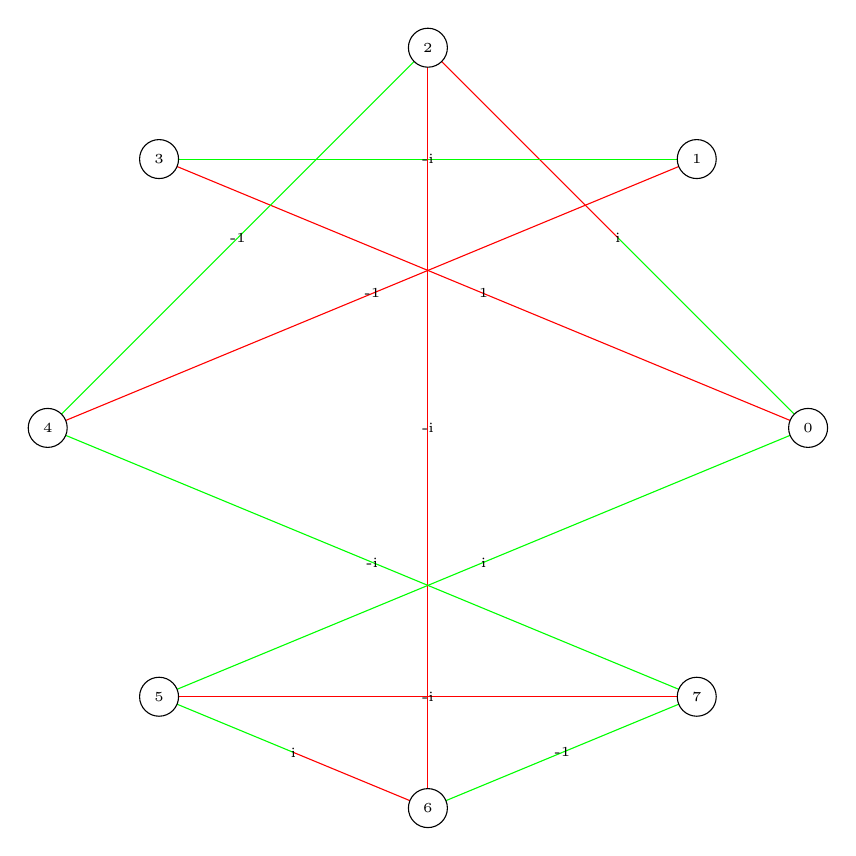
\begin{tikzpicture}
    \tikzstyle{every node}=[font=\tiny]
        \draw [style=thin, color=green] (4.82842712474619,0.0) to (2.414213562373095,2.414213562373095);
        \draw [style=thin, color=red] (2.414213562373095,2.414213562373095) to (2.9565589116183395e-16,4.82842712474619);
        \node [style=circle, draw=none] at (2.414213562373095,2.414213562373095) {i};
        \draw [style=thin, color=red] (4.82842712474619,0.0) to (0.7071067811865477,1.7071067811865475);
        \draw [style=thin, color=red] (0.7071067811865477,1.7071067811865475) to (-3.4142135623730945,3.414213562373095);
        \node [style=circle, draw=none] at (0.7071067811865477,1.7071067811865475) {1};
        \draw [style=thin, color=green] (4.82842712474619,0.0) to (0.707106781186547,-1.7071067811865472);
        \draw [style=thin, color=green] (0.707106781186547,-1.7071067811865472) to (-3.414213562373096,-3.4142135623730945);
        \node [style=circle, draw=none] at (0.707106781186547,-1.7071067811865472) {i};
        \draw [style=thin, color=green] (3.414213562373095,3.4142135623730945) to (2.220446049250313e-16,3.414213562373095);
        \draw [style=thin, color=green] (2.220446049250313e-16,3.414213562373095) to (-3.4142135623730945,3.414213562373095);
        \node [style=circle, draw=none] at (2.220446049250313e-16,3.414213562373095) {-i};
        \draw [style=thin, color=red] (3.414213562373095,3.4142135623730945) to (-0.7071067811865475,1.7071067811865475);
        \draw [style=thin, color=red] (-0.7071067811865475,1.7071067811865475) to (-4.82842712474619,5.913117823236679e-16);
        \node [style=circle, draw=none] at (-0.7071067811865475,1.7071067811865475) {-1};
        \draw [style=thin, color=green] (2.9565589116183395e-16,4.82842712474619) to (-2.414213562373095,2.4142135623730954);
        \draw [style=thin, color=green] (-2.414213562373095,2.4142135623730954) to (-4.82842712474619,5.913117823236679e-16);
        \node [style=circle, draw=none] at (-2.414213562373095,2.4142135623730954) {-1};
        \draw [style=thin, color=red] (2.9565589116183395e-16,4.82842712474619) to (-2.9565589116183395e-16,0.0);
        \draw [style=thin, color=red] (-2.9565589116183395e-16,0.0) to (-8.869676734855019e-16,-4.82842712474619);
        \node [style=circle, draw=none] at (-2.9565589116183395e-16,0.0) {-i};
        \draw [style=thin, color=green] (-4.82842712474619,5.913117823236679e-16) to (-0.7071067811865479,-1.7071067811865477);
        \draw [style=thin, color=green] (-0.7071067811865479,-1.7071067811865477) to (3.414213562373094,-3.414213562373096);
        \node [style=circle, draw=none] at (-0.7071067811865479,-1.7071067811865477) {-i};
        \draw [style=thin, color=green] (-3.414213562373096,-3.4142135623730945) to (-1.7071067811865483,-4.121320343559642);
        \draw [style=thin, color=red] (-1.7071067811865483,-4.121320343559642) to (-8.869676734855019e-16,-4.82842712474619);
        \node [style=circle, draw=none] at (-1.7071067811865483,-4.121320343559642) {i};
        \draw [style=thin, color=red] (-3.414213562373096,-3.4142135623730945) to (-8.881784197001252e-16,-3.414213562373095);
        \draw [style=thin, color=red] (-8.881784197001252e-16,-3.414213562373095) to (3.414213562373094,-3.414213562373096);
        \node [style=circle, draw=none] at (-8.881784197001252e-16,-3.414213562373095) {-i};
        \draw [style=thin, color=green] (-8.869676734855019e-16,-4.82842712474619) to (1.7071067811865466,-4.121320343559643);
        \draw [style=thin, color=green] (1.7071067811865466,-4.121320343559643) to (3.414213562373094,-3.414213562373096);
        \node [style=circle, draw=none] at (1.7071067811865466,-4.121320343559643) {-1};
        \node [style=circle, fill=white, draw=black] (0) at (4.82842712474619,0.0) {0};
        \node [style=circle, fill=white, draw=black] (1) at (3.414213562373095,3.4142135623730945) {1};
        \node [style=circle, fill=white, draw=black] (2) at (2.9565589116183395e-16,4.82842712474619) {2};
        \node [style=circle, fill=white, draw=black] (3) at (-3.4142135623730945,3.414213562373095) {3};
        \node [style=circle, fill=white, draw=black] (4) at (-4.82842712474619,5.913117823236679e-16) {4};
        \node [style=circle, fill=white, draw=black] (5) at (-3.414213562373096,-3.4142135623730945) {5};
        \node [style=circle, fill=white, draw=black] (6) at (-8.869676734855019e-16,-4.82842712474619) {6};
        \node [style=circle, fill=white, draw=black] (7) at (3.414213562373094,-3.414213562373096) {7};
    \end{tikzpicture}
    \caption{A perfectly monochromatic graph of size $8$ vertices, with a weighted matching index of $2$, discovered by EGPI during the experiment.}
    \label{fig:egpi_graph_example}
\end{figure}

From the results in figure~\ref{fig:results-experiment}, we can do the following observations.
Firstly, it is a lot harder to find perfectly monochromatic graphs in these conditions when their size is bigger.
Indeed, the number of possibilities grows exponentially with the number of vertices, and the probability to find a perfectly monochromatic graph decreases.
Secondly, the complexity bound has a big impact on the number of found graphs: a higher complexity bound results in a smaller number of found graphs.
This was expected, since the graphs generated with a higher complexity bound have higher chances to have more edges and perfect matchings.
The probability that all these randomly generated edges and perfect matchings together satisfy the definition~\ref{def:perfectly_monochromatic_graph} are small.\\

The last thing I am interested in is to count bipartite graphs among all the perfectly monochromatic graphs found.
The result is the following: \textbf{none} of the perfectly monochromatic graphs found were bipartite.
This is an alluring new observation: indeed, it is consistent with the arguments we used in the proofs of lemmas~\ref{lem:one_neg_edge} and~\ref{lem:2_positive_colour_classes_forbidden}.
One of the observations these proofs used is that, in these particular cases, the perfectly monochromatic graphs found were not bipartite.
This allows me to formulate the following conjecture.

\begin{conjecture}
    \label{con:bipartite_perfectly_monochromatic}
    Let $G_k^w$ be a non-redundant perfectly monochromatic graph that respects the following properties.
    \begin{itemize}
        \item $\Tilde{c}(G, k, w) \geq 2$
        \item $\forall e \in E(G_k^w), w(e) \in \{-1, 1, -i, i\}$
        \item $G_k^w$ has at least one non-monochromatic feasible vertex colouring.
    \end{itemize}
    Then, $G_k^w$ is not bipartite.
\end{conjecture}

This conjecture might constitute a new interesting subcase of the Krenn's conjecture to investigate in the future.


\section{Possible improvements for EGPI}
\label{sec:possible-improvements-for-egpi}

EGPI is a tool that can still be improved in many ways.\\

Firstly, currently it does not offer the functionality of generating only non-isomorphic graphs.
This functionality could be interesting if the user wants to count the number of different graphs generated by the tool.
This could be coded from scratch, or by using an external program.
For instance, in Python, the package \textit{NetworkX} offers a function to check if $2$ graphs are isomorphic or not~\cite{networkx}.
A more common program used a lot in the field of graph theory is Nauty, a program originally designed by Brendan McKay~\cite{MCKAY201494}.
Using it would offer a lot of advantages, but it would require to write a wrapper around it to use it in Python.
Indeed, Nauty is written in C. \\

A second improvement that could be brought to EGPI is to improve the efficiency of the algorithms used to find the perfect matchings of a graph.
Indeed, this step bounds the efficiency of most of the tasks performed by EGPI\@.
Improving this algorithm would allow the program to search more graphs in a given time, and to find more results in general.
One idea to improve it could be to look at the Edmonds' Blossom algorithm, an algorithm to find a single perfect matching in a graph~\cite{Edmonds_1965}.
It has to be determined whether this algorithm can be adapted to find all perfect matchings of a graph.\\
